\documentclass[11pt]{article}
\usepackage[margin=1in]{geometry}
\usepackage{amsmath,amssymb}
\usepackage{booktabs}
\usepackage{graphicx}
\usepackage[hidelinks]{hyperref}
\usepackage{xcolor}
\graphicspath{{../m1/figures/}{figures/}}

\title{MINERvA open-data sim$\to$reco surrogate:\\ performance report}
\author{L.~Wan\thanks{lwan@fnal.gov}}
\date{\today}

\begin{document}
\maketitle

\begin{abstract}
We document the performance of successive versions of a per-event surrogate that maps GENIE final-state
particles to MasterAnaDev reconstructed quantities, trained on the MINERvA open-data Medium Energy FHC Monte
Carlo. This version covers the M1 baselines: gradient-boosted trees for the reconstruction efficiency, MINOS
matching, muon charge and hadron-prong multiplicity, and mixture density networks for the muon momentum
response and the recoil energy. These numbers are the reference the generative model (M2) has to beat.
\end{abstract}

\section{Setup}
\label{sec:setup}

\paragraph{Data.} MINERvA open data~\cite{opendata}, Medium Energy FHC standard MC, playlist 1M, file
\texttt{run00113069}. The \texttt{Truth} tree holds every generated interaction; the \texttt{MasterAnaDev}
tree holds those with a reconstructed muon candidate together with a copy of the truth. The v1 training
population is CC $\nu_\mu$ interactions with true vertex $z \ge 4000$~mm; 39.6\% of them have a reco entry.

\paragraph{Inputs.} GENIE final-state particles after intranuclear FSI (\texttt{mc\_FSPart*}), dropping
neutrinos, neutrons, GENIE pseudo-particles and nuclear remnants, and hadrons with kinetic energy below
50~MeV. Each particle is a species class and $(p_x, p_y, p_z)$. The context is the true vertex $(x,y,z)$
and the struck nucleus $(Z, A)$. Generator-internal labels (interaction mode, $Q^2$, $W$, $E_\nu$) are
deliberately not used.

\paragraph{Splits.} Events are split by MC subrun (not by event) into train/validation/test:
\begin{center}\begin{tabular}{ccc}
\toprule
train & validation & test \\
\midrule
293537 & 37205 & 37654 \\
\bottomrule
\end{tabular}
\end{center}
All numbers below are on the test split.

\paragraph{Baseline features.} The M1 models use 48 hand-crafted event summaries (true muon momentum and
beam-frame angles; particle counts, summed and leading kinetic energies per species; leading-hadron angle
and class; hadronic $\sum p_T$; the context). The generative model of M2 will consume the particle set
directly.

\section{M1 baselines}
\label{sec:m1}

\subsection{Tier 0: efficiency, MINOS matching, charge}

Histogram-based gradient-boosted trees (\texttt{sklearn}, 15 leaves, learning rate 0.05, $\ell_2 = 1$,
early stopping). Table~\ref{tab:tier0} compares the test log loss to the marginal (constant-rate) predictor.

\begin{table}[h]\centering
\begin{tabular}{lcccc}
\toprule
Target & rate & log loss (marginal) & log loss (GBDT) & AUC \\
\midrule
reconstructed (muon candidate) & 0.397 & 0.6718 & 0.4229 & 0.882 \\
MINOS matched $\mid$ reconstructed & 0.787 & 0.5173 & 0.1015 & 0.987 \\
negative charge $\mid$ matched & 0.965 & 0.1506 & 0.1272 & 0.795 \\
\bottomrule
\end{tabular}

\caption{Tier 0 binary targets. Lower log loss is better; the marginal column is the constant predictor.}
\label{tab:tier0}
\end{table}

\begin{figure}[h]\centering
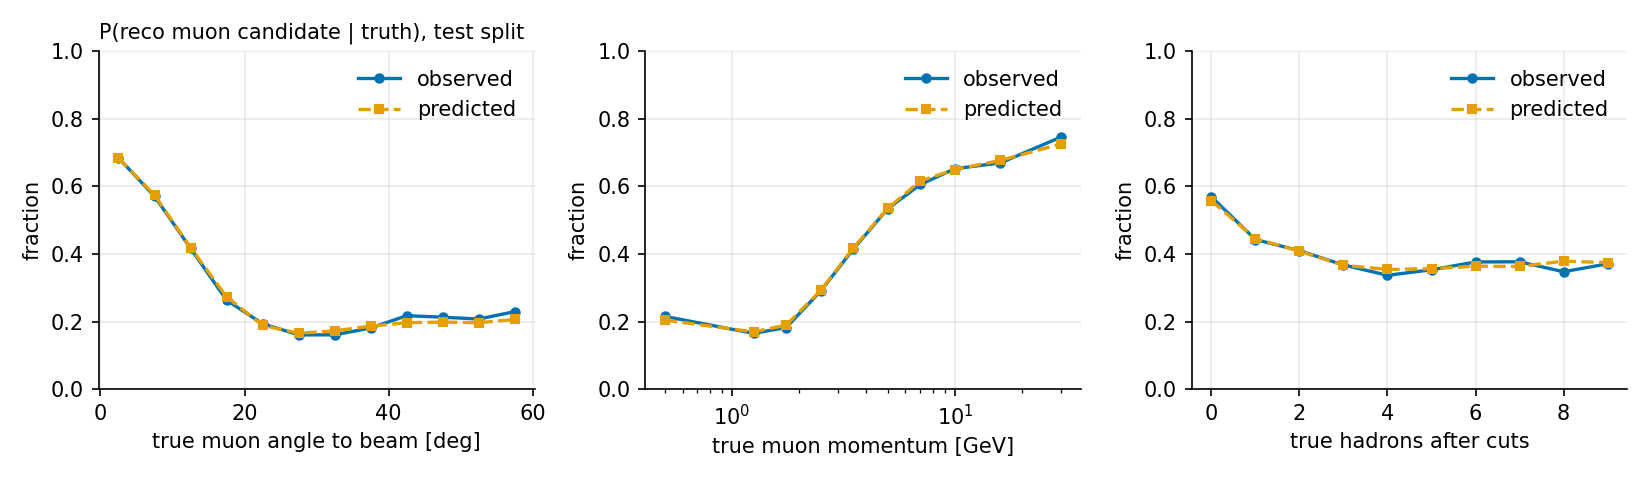
\includegraphics[width=\textwidth]{m1_efficiency_calibration.png}
\caption{Observed versus GBDT-predicted probability that a CC~$\nu_\mu$ event has a reconstructed muon
candidate, in bins of true muon angle, true muon momentum, and number of hadrons after cuts.}
\label{fig:eff}
\end{figure}

\begin{figure}[h]\centering
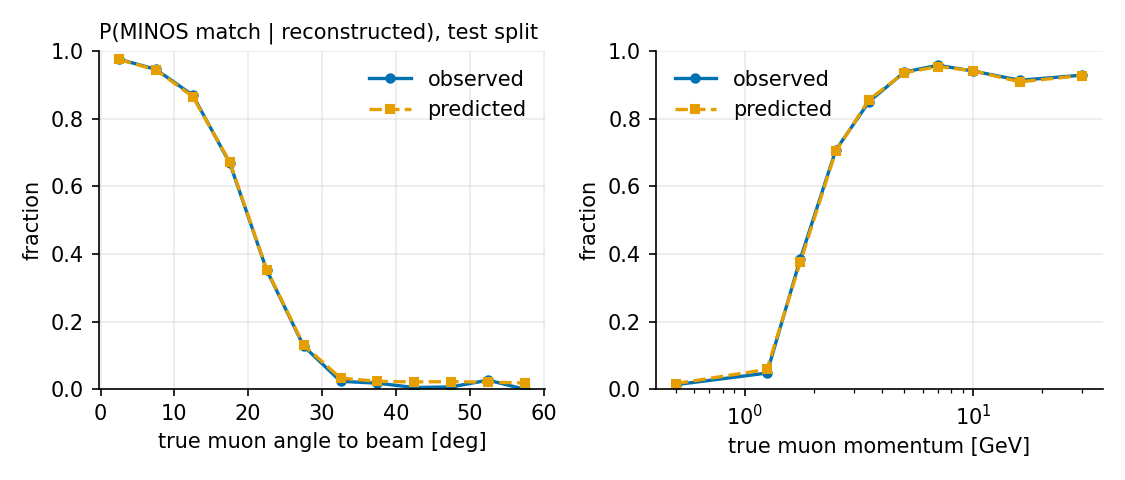
\includegraphics[width=0.7\textwidth]{m1_minos_calibration.png}
\caption{Observed versus predicted MINOS-match probability among reconstructed events.}
\label{fig:minos}
\end{figure}

\subsection{Hadron-prong multiplicity}

Multiclass GBDT over $n_\mathrm{prongs} \in \{0,\dots,5,6{+}\}$ among reconstructed events. Sampled
multiplicities are drawn from the predicted class probabilities.

\begin{table}[h]\centering
\begin{tabular}{lcc}
\toprule
 & marginal & GBDT \\
\midrule
log loss & 1.0632 & 0.8432 \\
accuracy & 0.441 & 0.624 \\
\bottomrule
\end{tabular}

\caption{Multiplicity classifier versus the marginal distribution.}
\label{tab:mult}
\end{table}

\begin{table}[h]\centering
\begin{tabular}{lccccccc}
\toprule
true $\backslash$ sampled & 0 & 1 & 2 & 3 & 4 & 5 & 6+ \\
\midrule
0 & 0.60 & 0.32 & 0.07 & 0.01 & 0.00 & 0.00 & 0.00 \\
1 & 0.32 & 0.54 & 0.12 & 0.02 & 0.00 & 0.00 & 0.00 \\
2 & 0.24 & 0.48 & 0.22 & 0.05 & 0.01 & 0.00 & 0.00 \\
3 & 0.29 & 0.44 & 0.19 & 0.07 & 0.00 & 0.00 & 0.00 \\
4 & 0.19 & 0.48 & 0.31 & 0.02 & 0.00 & 0.00 & 0.00 \\
5 & 0.14 & 0.57 & 0.29 & 0.00 & 0.00 & 0.00 & 0.00 \\
6+ & 0.00 & 0.67 & 0.33 & 0.00 & 0.00 & 0.00 & 0.00 \\
\bottomrule
\end{tabular}

\caption{Row-normalised confusion between true and sampled reco multiplicity (test split).}
\label{tab:mult-conf}
\end{table}

\begin{figure}[h]\centering
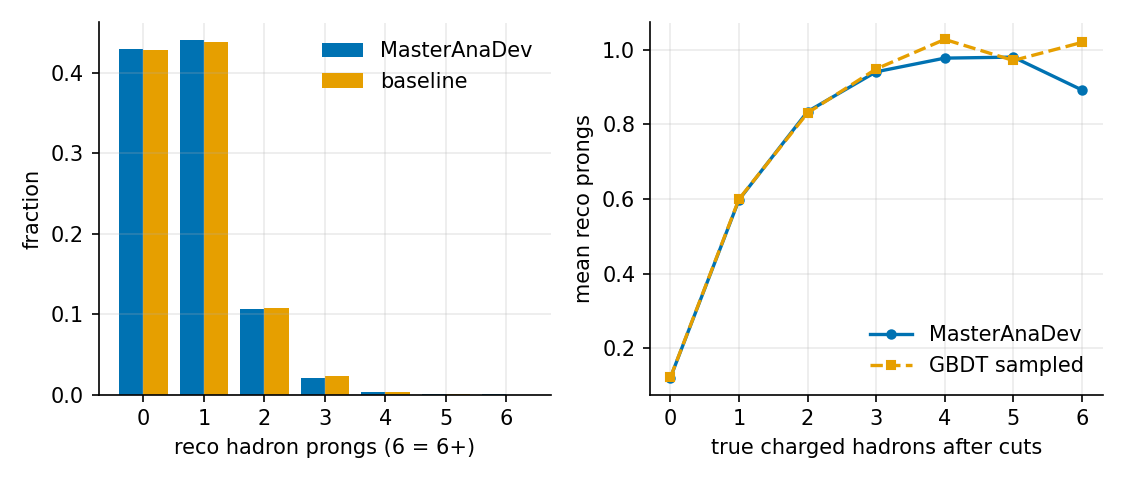
\includegraphics[width=0.7\textwidth]{m1_multiplicity.png}
\caption{Left: marginal reco prong multiplicity, MasterAnaDev versus GBDT samples. Right: mean reco prongs
versus true number of charged hadrons after cuts.}
\label{fig:mult}
\end{figure}

\subsection{Muon response and recoil energy: mixture density networks}

An MDN with $K$ diagonal-Gaussian components, three hidden layers of 256 units, conditioned on the
standardised features plus the MINOS-match flag. Targets: $\log(P_\mathrm{reco}/P_\mathrm{true})$ and the
two slope differences $\Delta(p_x/p_z)$, $\Delta(p_y/p_z)$ for the muon; $\log E_\mathrm{recoil}$ for the
calorimetric recoil. $K=1$ is a heteroscedastic Gaussian regression; $K=8$ is the baseline proper.

\begin{table}[h]\centering
\begin{tabular}{lcc}
\toprule
Target & Gaussian ($K=1$) & MDN ($K=8$) \\
\midrule
muon response (3-d) & -4.2164 & -5.5104 \\
$\log E_\mathrm{recoil}$ (1-d) & 0.8526 & 0.7116 \\
\bottomrule
\end{tabular}

\caption{Test negative log-likelihood per event (natural log, original units). Lower is better.}
\label{tab:nll}
\end{table}

\begin{table}[h]\centering\small
\resizebox{\textwidth}{!}{\begin{tabular}{lccc}
\toprule
Variable & MasterAnaDev median [16\%, 84\%] & MDN sample median [16\%, 84\%] & $W_1$ \\
\midrule
muon $\log(P_\mathrm{reco}/P_\mathrm{true})$, MINOS matched & -0.004 [-0.102, 0.079] & -0.001 [-0.095, 0.084] & 0.0084 \\
muon $\log(P_\mathrm{reco}/P_\mathrm{true})$, not matched & -0.564 [-1.988, 0.950] & -0.606 [-1.973, 0.964] & 0.0477 \\
muon $\Delta(p_x/p_z)$ & 0.000 [-0.015, 0.014] & -0.000 [-0.014, 0.014] & 0.0844 \\
muon $\Delta(p_y/p_z)$ & 0.000 [-0.014, 0.015] & -0.000 [-0.014, 0.015] & 0.0883 \\
$\log(E_\mathrm{recoil}/\mathrm{MeV})$ & 7.485 [6.077, 8.558] & 7.469 [6.069, 8.528] & 0.0193 \\
\bottomrule
\end{tabular}
}
\caption{Marginal distributions of MasterAnaDev versus one MDN ($K=8$) sample per test event, and the
1-Wasserstein distance between them (same units as the variable).}
\label{tab:mdn-marg}
\end{table}

\begin{figure}[h]\centering
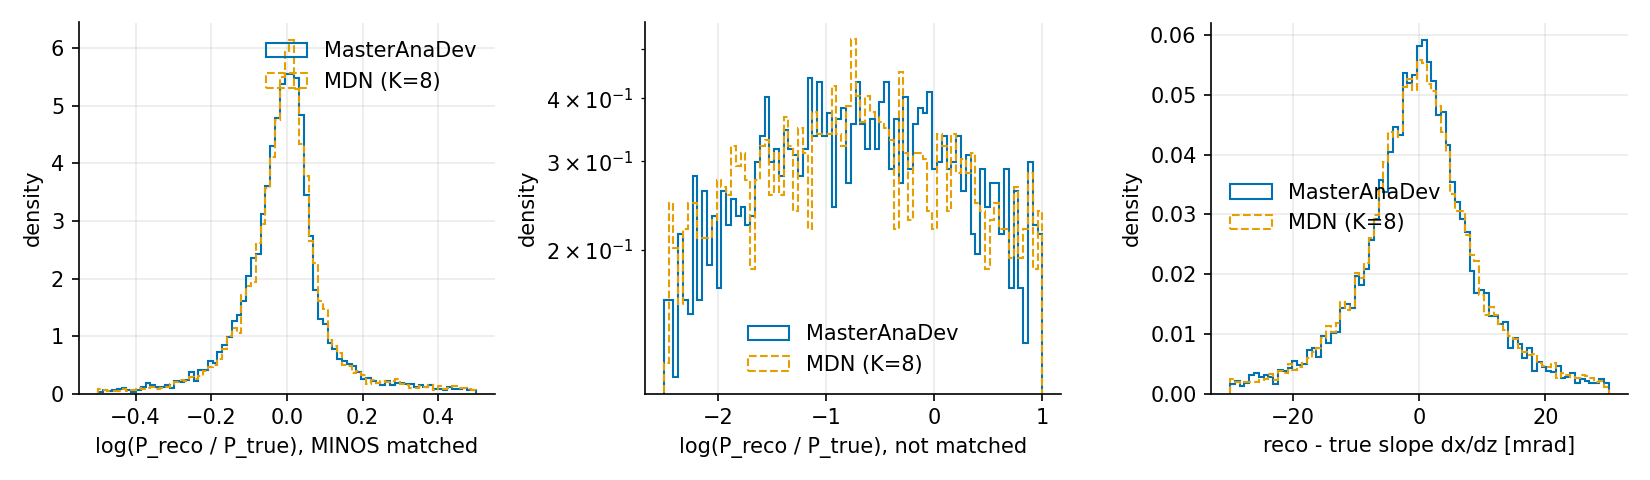
\includegraphics[width=\textwidth]{m1_muon_response.png}
\caption{Muon response, test split: momentum ratio for MINOS-matched and unmatched muons, and the $x$-slope
difference.}
\label{fig:muon}
\end{figure}

\begin{figure}[h]\centering
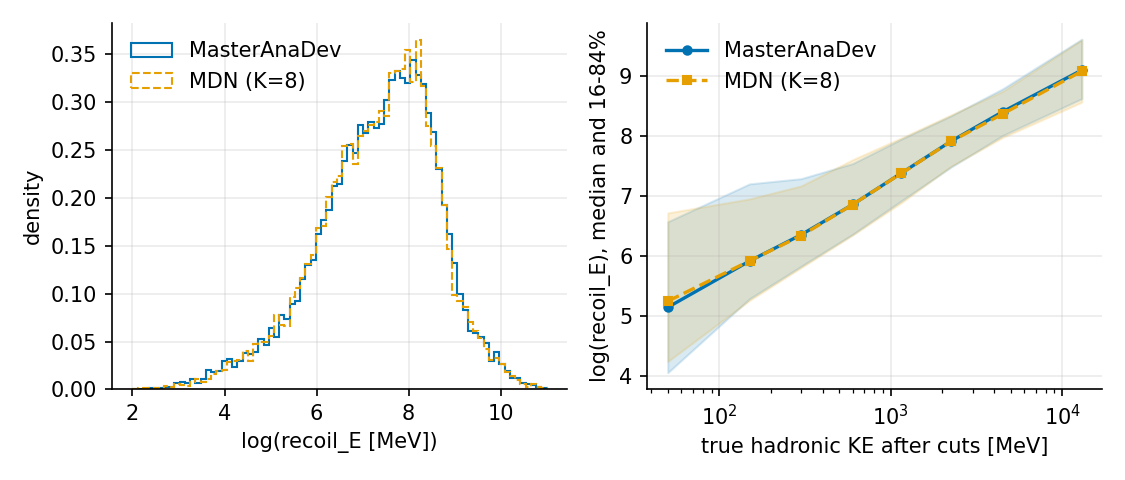
\includegraphics[width=0.7\textwidth]{m1_recoil.png}
\caption{Recoil energy: marginal (left) and median with 16--84\% band versus true hadronic kinetic energy
after cuts (right).}
\label{fig:recoil}
\end{figure}

\section{Discussion}
\label{sec:discussion}
The baselines set three kinds of reference for the generative model.

\paragraph{What is already easy.} MINOS matching is almost a deterministic function of the true muon
kinematics: the tree reaches AUC~0.987 and cuts the log loss from 0.52 to 0.10. The reconstruction
efficiency is predicted without visible bias across muon angle, muon momentum and hadron count
(Fig.~\ref{fig:eff}); its residual log loss (0.42 versus 0.67 marginal) is irreducible randomness in
whether a muon track is found, not a modelling deficit. The recoil-energy median follows the true hadronic
kinetic energy over two decades and the MDN reproduces the 16--84\% band (Fig.~\ref{fig:recoil}).

\paragraph{What needs a proper generative model.} The muon momentum response is bimodal in the sense that
matters for analyses: MINOS-matched muons have a $\pm 9\%$ core, unmatched muons a spread of more than a
factor two in either direction. The $K=1$ Gaussian cannot represent this (Table~\ref{tab:nll}); the
$K=8$ MDN does, with $W_1 = 0.008$ in $\log(P_\mathrm{reco}/P_\mathrm{true})$ for matched and $0.05$ for
unmatched muons. But the MDN sees only 48 summary features. Correlations between the muon response, the
recoil energy and the prong content of the same event are not modelled at all here, and these are exactly
what a cross-section analysis with a multi-variable signal definition depends on. That joint structure is the
job of the M2 flow-matching model over the particle set.

\paragraph{Where the baseline is weak.} Multiplicity is the hardest target so far. The tree beats the
marginal (log loss 0.84 versus 1.06, accuracy 0.62 versus 0.44) and reproduces the mean reco prongs versus
true charged hadrons up to three hadrons (Fig.~\ref{fig:mult}), but the confusion table shows that events
with four or more true charged hadrons are still mostly assigned one or two prongs, with the saturation at
high multiplicity slightly overshot. Whether the saturation is learnable from the particle set rather than
from counts is one of the questions the M2 model must answer; it also bears directly on the extrapolation
study, since high-multiplicity final states are where alternative generators differ most.

\paragraph{Caveats.} All numbers are from a single MC file (368k CC~$\nu_\mu$ events, 39.6\% reconstructed)
and a single seed. Test negative log-likelihoods for the muon MDN are quoted with the same $\pm 25\sigma$
robust clipping used in training; without it a handful of muons with $|p_x/p_z| \gg 1$ dominate the mean.
The features exclude generator-internal labels by design, so nothing here would change for another
generator's final states, but neither has that transfer been tested yet: the extrapolation holdouts of
the design document (train on QE+RES+2p2h, test on DIS; train on $\le 2$ visible hadrons, test on more)
are scheduled for M3.


\begin{thebibliography}{9}
\bibitem{opendata} MINERvA Collaboration, Open Data Release, \url{https://minerva.fnal.gov/opendata/},
\href{https://doi.org/10.15484/3022562}{doi:10.15484/3022562}.
\end{thebibliography}

\end{document}
